\chapter{Research}


\section{History}

In 1736, \citet{euler} solved the Seven Bridges of Ka\"{o}nigsberg problem by drawing a graph.
\citet{ismail2009some}
\todo{a strange paper to choose. perhaps multiple citations?}
pinpoint his use of this method as the birth of graph theory.

Graph theory has many applications to modelling the real world \ldots

\subsection{Tutte-embeddings}

In 1963, \citet{tutte} popularised [says who] the problem of graph drawing when he presented 

["who showed that polyhedral graphs may be drawn in the plane with all faces convex by fixing the vertices of the outer face of a planar embedding of the graph into convex position, placing a spring-like attractive force on each edge, and letting the system settle into an equilibrium"]

This contained two important ideas: embeddings(, , and the application of an attractive spring-like attractive force \ldots 

\subsection{Knuth}

In the same year, \citet{Knuth63} described a system for drawing flowcharts that describe algorithms. \citet{battista} \todo{find out page number!} says this is [the first example of an algorithm for visualising information] although \citeauthor{Knuth63} cites earlier work done on a similar system by \citet{haibt1959}.

\citet{Knuth63} does not describe his flowcharts as graphs,

The annual symposium is 


\ldots

\citet{huang2007effects} divide graphs into two groups: abstract graphs and domain graphs.
GSN arguments fall into the latter category \ldots  therefore \ldots
\todo{I don't think this is widely agreed upon}







\section{What makes a good graph layout?}

The GSN was intended to be a clearer way of presenting arguments than free text.
The simple act of breaking down arguments into their constituent parts achieves some of this clarity,
but the notation's graphical nature also appears to be important.
This raises the question of whether the particular layout of graphs can affect their comprehensibility.

\subsection{Common goals}

\citet{DiBattista1997303} compared 4 algorithms, by using implementations of them to lay out 11,582 graphs generated from 112 real life applications. They compared the resulting layouts, based on nine quality metrics:

\begin{description}
\item[Area]
``area of the smallest rectangle with horizontal and vertical sides covering the drawing''
\item[Cross]
total number of edge crossings
\item[TotalBends]
total number of edge bends
\item[TotalEdgeLen]
total length of all edges
\item[MaxEdgeBends]
``maximum number of bends on any edge''
\item[MaxEdgeLen]
``maximum length of any edge''
\item[UnifBends]
``standard deviation of the number of bends on the edges''
\item[UnifLen]
``standard deviation of the edge length''
\item[ScreenRatio]
``deviation from the optimal aspect ratio, computed as the difference between the width/height ratio of the best of the two possible orientations (portrait and landscape) of the drawing and the standard 4/3 ratio of a computer screen. ''
\end{description}

They boldly assert: ``It is widely accepted \ldots that small values of the above measures are related to the perceived aesthetic appeal and visual effectiveness of the drawing.''
But widely accepted things can be wrong. \todo{Galileo, Copernicus!?}

The \textbf{ScreenRatio} metric is perhaps the [superlative] [adjective], because statistics such as those published by Unity Technologies\footnote{\url{http://stats.unity3d.com/}} show that 4:3 is no longer the most common computer screen aspect ratio. 
Furthermore, and , a desirable aspect ratio . If aesthetic beauty is important, then perhaps the golden ratio 
Being only one metric of nine, it is not given undue significance, but it might be better ignored altogether.

Aesthetic appeal is likely to satisfy users of tools such as Artoo, making them less inclined to manually adjust layouts.

It is tempting to assume that the seemingly highly prized characteristics of layouts produced by certain algorithms are always relevant. After all, why else would they be stated as advantages? However, graph theory -- and, in turn, graph layout -- has a broad range of applications. \todo{Literature does not always fully the advantages of layouts' advantages \ldots does it?}

For example, there can be many practical motivations for minimising edge crossings.
When P\`{a}l Tur\`{a}n worked in a brick factory during World War II,
he considered the minimum number of crossings in a graph representing
brick kilns, storage sites and the paths between them \todo{cite}.
Where a graph represents an electrical circuit, edge crossings affect how the circuit can be printed on a circuit board.

Therefore, seemingly desirable characteristics of layouts produced by certain algorithms are not always relevant to a particular application.
Clearly, the characteristics of a layout algorithm suitable for GSN arguments must \ldots

\subsection{Gestalt principles}


The Gestalt principles of visual perception,
based on the wider Gestalt theory of the mind developed by German psychologists of the Berlin School in the late 19th and early 20th centuries,
are sometimes [?] used to [inform/justify?] graph layouts.

The principle 

The relationship between the Gestalt principles and \ldots can seem hazy and tenuous

\subsection{The human gold-standard \todo{could move this above 2.2.1}}

One understanding of the ideal layout of a GSN argument can be reached by observing manually layed out arguments ``in the wild''.
Examples can be found in literature, such as \citet{insilico}, \citet{Habli:2006:PPC:1183088.1183090} \ldots

Layouts typically follow the guidelines described in the GSN specification \citep[section~2.2, pp.~26--27]{gsnstandard}, to ``enable the reader to perceive the logical flow of the argument being presented, and to enhance its readability.''
Although the specification document does not fully justify its recommendations, they seem reasonable.

The specification suggests that arguments should flow down the page, starting with an abstract parent goal at the top, progressing downwards as this is refined into more concrete child strategies, goals and solutions -- this allows the hierarchy of the graph to be understood without looking at the directions of the connecting arrows.
Context and justification elements are placed off to the sides, a positioning which reflects their semantic role.

The layout guidance is not demonstrated with specific diagrams, but there are many examples elsewhere in the document.
These follow the guidelines, but . As discussed in, the layout shown in figure~\ref{fig:crampedex1} is more cramped than it could be.
Another example, shown in figure~\ref{fig:unaligned_siblings}, ignores \todo{I think ``violates'' would be wrong} Gestalt  \ldots
This leads to the conclusion that, although examples found in literature are not always are perfectly laid out, the imperfections are often easy to identify.

\begin{figure}
    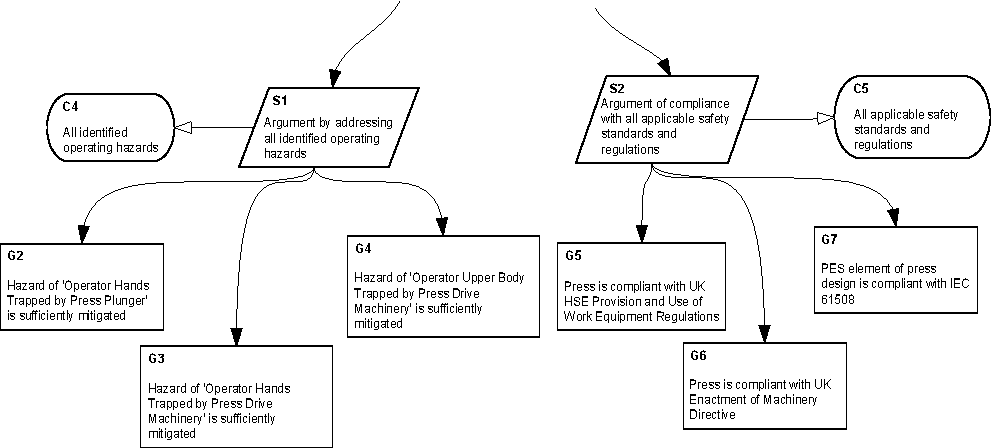
\includegraphics[width=\textwidth]{graphics/unaligned_siblings.pdf}
    \caption{A fragment of a GSN argument,
            from the GSN specification \citep[figure~42, section~2.3.6.5, pp.~34]{gsnstandard}}
    \label{fig:unalignedsiblings}
\end{figure}

\begin{figure}
    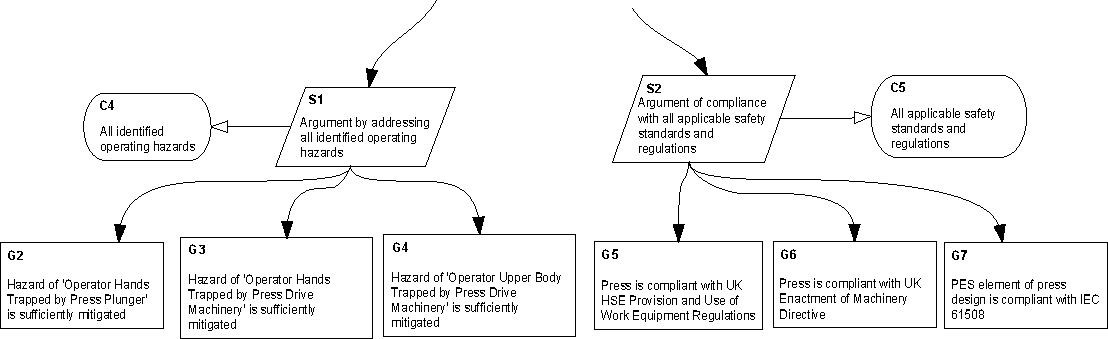
\includegraphics[width=\textwidth]{graphics/aligned_siblings.pdf}
    \caption{A modified version of figure~\ref{fig:unalignedsiblings},
            showing more clearly that the six goal elements are at the same level in the hierarchy}
    \label{fig:alignedsiblings}
\end{figure}


\subsection{Experimental comparison} 

\citeauthor{DiBattista1997303}

Some studies have looked a the  \ldots cognitive effects [Purchase et al?]

characterising 


\subsection{Edge crossings}


[But] more relevantly [which studies?] have found that edge crossings is the most important factor for comprehension

[who?] found that using the Gestalt principle of `closure' \ldots the viewer's mind instinctively joins up the lines




\section{Approaches to graph layout}

\subsection{Force directed algorithms}

Force directed graph layout algorithms are the descendants of \todo{as someone has observed?} \citet{tutte} \ldots a successor to \citet{tutte} spring embedding.

Force directed layout is simple to understand, being based on physical laws we encounter in the world 


[gansner 199*]

\subsection{grid}




\subsection{Layered graph drawing}

Layered or hierarchical graph drawing  \ldots sometimes generalised as Sugiyama's method, after \ldots who pioneered this technique \ldots 




\section{[GSN-/Artoo-specific considerations?]}

[move to Requirements?]

The  \ldots



\subsection{Dangling edges}

suggests incomplete graph

\subsection{Directed cycles}

It can be useful to remove directed cycles from the internal representation of a graph
(before drawing them back in their correct, original directions)
-- for example, in order to assign a consistent rank to each node.
This is achieved by reversing certain edges.
\citet{gansner1993} show that a simple depth-first-search \ldots  Minimising the number of edges is more difficult, \citeauthor{gansner1993} \ldots

\subsection{Undirected cycles}

Undirected cycles can be eliminated by ignoring certain edges altogether, to produce a tree.  [citation needed]








\section{Implementation}

The Artoo tool is written mainly in JavaScript, numerous different 

Various [things] have been developed in response to perceived shortcomings in JavaScript \ldots

Programs written in the CoffeeScript\footnote{\url{http://coffeescript.org/}} language, designed to be more succinct and with some extra features, can be transcompiled to JavaScript \ldots this is interesting but \ldots

Brython \footnote{\url{http://www.brython.info/}} is a Python 3 interpreter written in JavaScript that can run in a web browser. \todo{performance overhead etc\ldots}

Haste\footnote{\url{http://haste-lang.org/}}, UHC-JS\footnote{\url{http://uu-computerscience.github.io/uhc-js/}} and GHCJS\footnote{} are compilers from Haskell to JavaScript; SMLtoJS\footnote{\url{http://www.smlserver.org/smltojs/}} is a Standard ML--to-JavaScript compiler. These are perhaps most interesting [?], since \citet{kennedyfuntrees} observed that a tree layout algorithm implemented in Standard ML ``reflects the structure of the abstract solution much better than an imperative language implementation''.



ASM\footnote{} is a strict subset of 

[However]


\section{Software development methodologies}

In \citeyear{67poorslop}, \citet*{67poorslop} explained ``Why Programming is a Good Medium for Expressing Poorly Understood and Sloppily Formulated Ideas''
(More recently, [sussman] gave a talk with the same title \ldots \todo{\url{http://vimeo.com/12060509}}.)

This idea will be 

\section{}

Reuse of existing software libraries is widely [?] understood to be [a very sensible idea]. There are , which \ldots for comparison with 

\begin{description}
  \item[Springy] is 
  \item[Arbor] is an implementation of the Barnes-Hut algorithm described in  
  \item[The JavaScript InfoVis Toolkit] contains algorithms ported from \ldots
  \item[vis.js]
\end{description}

The Graphviz library contains several algorithms, including \ldots [as described in \ldots]. Although it is written in C, Emscripten \footnote{\url{http://emscripten.org}} can compile LLVM bitcode (readily compiled from C code) [as described earlier?] to the ASM subset of JavaScript -

These implementations also provide lessons on the structure of \ldots



agile
